% !TEX TS-program = xelatex+makeindex+bibtex+shellescape
% !TEX encoding = UTF-8 Unicode

% This file is a template using the "beamer" package to create slides for a talk or presentation
% - Giving a talk on some subject.
% - The talk is between 15min and 45min long.
% - Style is ornate.

% MODIFIED by Jonathan Kew, 2008-07-06
% The header comments and encoding in this file were modified for inclusion with TeXworks.
% The content is otherwise unchanged from the original distributed with the beamer package.

\documentclass{beamer}


% Copyright 2004 by Till Tantau <tantau@users.sourceforge.net>.
%
% In principle, this file can be redistributed and/or modified under
% the terms of the GNU General Public License, version 2.
%
% However, this file is supposed to be a template to be modified
% for your own needs. For this reason, if you use this file as a
% template and not specifically distribute it as part of a another
% package/program, I grant the extra permission to freely copy and
% modify this file as you see fit and even to delete this copyright
% notice. 


\mode<presentation>
{
  \usetheme{Warsaw}
  % or ...

  % \setbeamercovered{transparent}
  % or whatever (possibly just delete it)
}
\usefonttheme[onlymath]{serif}
\setbeamertemplate{caption}[numbered]
\setbeamerfont{footnote}{size=\tiny}


\usepackage[english]{babel}
%\usepackage{enumitem}
\usepackage{environ}
\usepackage{pgffor}
\usepackage{minted}
\usepackage{pgfplots}
\pgfplotsset{height=0.8\textheight,compat=1.9}

% or whatever

\usepackage[utf8]{inputenc}
% or whatever

\usepackage{times}
\usepackage[T1]{fontenc}
% Or whatever. Note that the encoding and the font should match. If T1
% does not look nice, try deleting the line with the fontenc.

\newcounter{boxCounter}
\newsavebox{\boxA}
\newsavebox{\boxB}
\newsavebox{\boxC}
\newsavebox{\boxD}


\newlength{\availafter}

\NewEnviron{autotext}[1][0.5cm]
{\setcounter{boxCounter}{0}\foreach \mysize in {\normalsize,\small,\footnotesize,\scriptsize}{\stepcounter{boxCounter}\expandafter\savebox\csname box\Alph{boxCounter}\endcsname{\vbox{\mysize\BODY}}\setlength{\availafter}{\dimexpr\textheight-\expandafter\ht\csname box\Alph{boxCounter}\endcsname-\pagetotal\relax}\ifdim\availafter>#1\expandafter\usebox\csname box\Alph{boxCounter}\endcsname\breakforeach\fi}}



\title[PHYS-2211-Lab01] % (optional, use only with long paper titles)
{Physics 2211 - Lab 1}

\subtitle
{Constant Velocity Motion} % (optional)

\author[Menon, Advaith] % (optional, use only with lots of authors)
{Advaith~Menon\inst{1}}
% - Use the \inst{?} command only if the authors have different
%   affiliation.

\institute%[Universities of Somewhere and Elsewhere] % (optional, but mostly needed)
{
  \inst{1}%
  Computer Engineering\\
  Georgia Institute of Technology
  }
% - Use the \inst command only if there are several affiliations.
% - Keep it simple, no one is interested in your street address.

\date%[Short Occasion] % (optional)
{January 25\textsuperscript{th}, 2023}

\subject{Talks}
% This is only inserted into the PDF information catalog. Can be left
% out. 



% If you have a file called "university-logo-filename.xxx", where xxx
% is a graphic format that can be processed by latex or pdflatex,
% resp., then you can add a logo as follows:

% \pgfdeclareimage[height=0.5cm]{university-logo}{university-logo-filename}
% \logo{\pgfuseimage{university-logo}}



% Delete this, if you do not want the table of contents to pop up at
% the beginning of each subsection:
%\AtBeginSubsection[]
\AtBeginSection[]
{
  \begin{frame}<beamer>{Outline}
    \tableofcontents[currentsection,currentsubsection]
  \end{frame}
}


% If you wish to uncover everything in a step-wise fashion, uncomment
% the following command: 

%\beamerdefaultoverlayspecification{<+->}


\begin{document}

\begin{frame}
  \titlepage
\end{frame}

\begin{frame}{Outline}
  \tableofcontents
  % You might wish to add the option [pausesections]
\end{frame}


% Since this a solution template for a generic talk, very little can
% be said about how it should be structured. However, the talk length
% of between 15min and 45min and the theme suggest that you stick to
% the following rules:  

% - Exactly two or three sections (other than the summary).
% - At *most* three subsections per section.
% - Talk about 30s to 2min per frame. So there should be between about
%   15 and 30 frames, all told.

\section{Introduction}
\subsection[Aim]{Aim of the experiment}
\begin{frame}{Aim}{Purpose of this lab assignment}
	\begin{itemize}
	\item Observe the motion of some object that is moving at the same speed without changing direction
	\item Analyzing the motion using software tools (Tracker) and capturing the object's positions at uniform time intervals.
	\item Creating a computational model using VPython to represent and predict motion in this situation, and compare it with actual data from Tracker.
	\end{itemize}
\end{frame}

\section{Prerequisites}
\subsection{Newton's First Law}
\begin{frame}{Newton's First Law}{Qualitative analysis of motion}
	``Every body persists in its state of being at rest
	or of moving uniformly straight forward, except
	insofar as it is compelled to change its state by
	force impressed.''
\end{frame}

\begin{frame}{Newton's Second Law}{Quantitative analysis of motion}
	``The net force acting on a body is defined as the change in its 
	momentum per unit time.''
	\begin{equation}
	\vec{F}_{net} = \frac{\mathrm{d}\vec{p}}{\mathrm{d}t}
	\end{equation}
	In most daily life scenarios, mass doesn't change with respect to
	time, hence this equation is better known as:
	\[\vec{F}_{net} = m\cdot\vec{a}\]
	where,
	\begin{itemize}
	\item \(\vec{F}_{net} = \) Net force acting on a body
	\item \(m = \) Mass of the body
	\item \(\vec{a} = \frac{\mathrm{d}\vec{v}}{\mathrm{d}t} 
		= \frac{\mathrm{d}^2\vec{r}}{\mathrm{d}t^2} = \) 
		Net acceleration on body	
	\item \(\Delta\vec{p} = m\times\Delta\vec{v} = \)
		Change in momentum
	\end{itemize}
\end{frame}

\subsection{Initial conditions, system and surroundings}
\begin{frame}{Initial conditions}
	\begin{itemize}
	\item \(\vec{r} = \vec{0} \), where \(\vec{r}\) stands for position vector
	\item \(\vec{F}_{net} = \vec{0}\)
	\item \(\vec{v}_i \neq \vec{0} \), we have to calculate this!
	\end{itemize}
\end{frame}

\begin{frame}{System and surroundings}
	\begin{itemize}
	\item \textbf{System:} Aerosol can (hereafter referred to as `object')
	\item \textbf{Surroundings:} Everything else (table, air, etc.)
	\end{itemize}
\end{frame}

\section{Experiment}
\subsection{Observation using Video}
\begin{frame}{Analysis of Video}{Getting displacement at discrete time intervals using Tracker}
\begin{figure}
\centering
    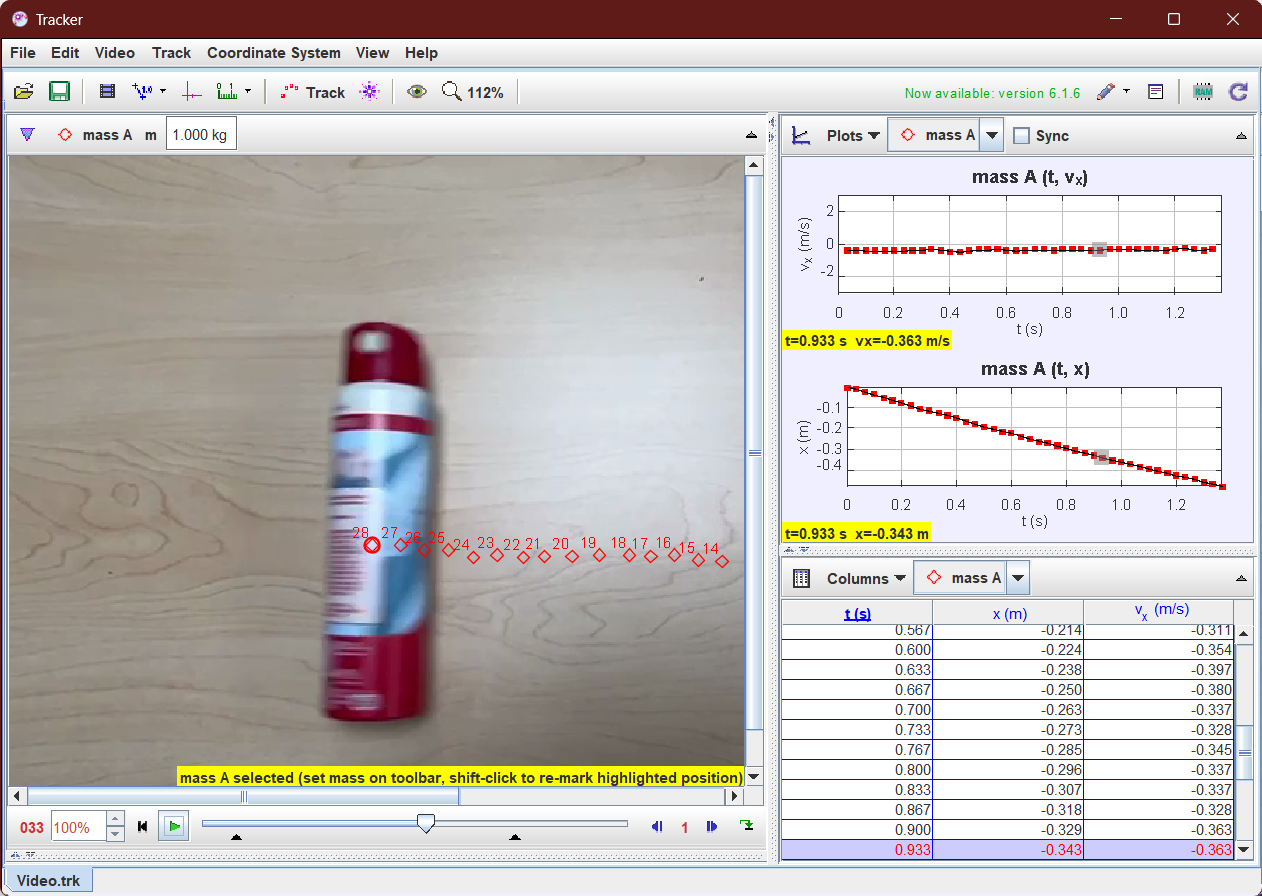
\includegraphics[height=0.7\textheight]{res/trackerScreenShot}
    \caption{Using Tracker\textsuperscript{\textregistered} to analyze the motion of the object.}
    \label{fig:trackerSS}
\end{figure}
\end{frame}

\begin{frame}{Calculating Velocity}
\begin{columns}
\begin{column}{0.5\textwidth}
   \begin{center}
   \begin{tabular}{|r|r|}
   \hline
   \textbf{Time} \(t\) (s) & \textbf{X-Position} \(r_x\) (m) \\
   \hline
   \(0.00\times 10^0\) & \(-2.88\times 10^{-3}\) \\
   \hline
   \(3.33\times 10^{-2}\) & \(-1.32\times 10^{-2}\) \\
   \hline
   \(6.67\times 10^{-2}\) & \(-2.59\times 10^{-2}\) \\
	\hline
	\(1.00\times 10^{-1}\) & \(-3.86\times 10^{-2}\) \\
	\hline
	\(1.33\times 10^{-1}\) & \(-5.18\times 10^{-2}\) \\
	\hline
	\multicolumn{2}{|c|}{\vdots\ \ \ \ \ \ \ \ \ \ \ \ \vdots} \\
	\hline
   \end{tabular}
   \end{center}
\end{column}
\begin{column}{0.5\textwidth}
	\begin{itemize}
		\item \[\vec{v}_{avg} = \frac{\vec{r}_2-\vec{r}_1}
				{t_2-t_1}\]
		\item The average velocity of the first two rows is\footnote{The i-j-k hat 
				notation for vectors has been used due to paucity of space.}:
				\(\vec{v}_{avg} = \frac{-1.32\times 10^{-2}\hat{i}\ \mathrm{m}-(-2.88\times 10^{-3}\hat{i}\ \mathrm{m})}
				{3.33\times 10^{-2}\ \mathrm{s}-0} = -3.11\times 10^{-1}\ \mathrm{ms^{-1}}\)
	\end{itemize}
\end{column}
\end{columns}
\end{frame}

\begin{frame}{Calculating Velocity}
\begin{columns}
\begin{column}{0.5\textwidth}
	\begin{autotext}
   \begin{itemize}
	\item Repeating this step multiple times, we can get the average
		velocity for each interval
	\item Ideally, the average velocity for each interval should be 
		constant, but due to various factors such as air resistance
		, friction on the surface, etc, the velocity is not constant. 
	\item Hence, we average the velocities of these small steps to get an 
	accurate reading.
	\end{itemize}
	\end{autotext}
\end{column}
\begin{column}{0.5\textwidth}
	\begin{figure}
	\centering
	    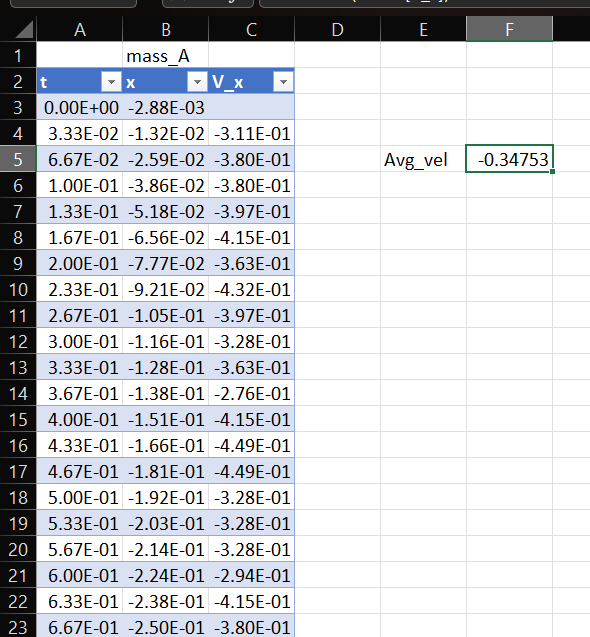
\includegraphics[height=0.6\textheight]{res/excelValueSS}
	    \caption{Using Excel to calculate average velocity}
	    \label{fig:trackerSS}
	\end{figure}
\end{column}
\end{columns}
\end{frame}
\subsection{Computational Model}

\begin{frame}{Data}{Data needed for simulation}
\begin{itemize}
\item Velocity of object at given instant \( = -0.34753\)
 ms\textsuperscript{-1}
\item Total time \( = 1.37\)s
\item Initial position \( = \vec{0} \)
\end{itemize}
\end{frame}

\begin{frame}[fragile]{Code}{Simulating the constant velocity}
\begin{minted}[breaklines]{python}
ball = sphere(color=color.blue, radius=0.22) 
trail = curve(color=color.green, radius=0.02)
origin = sphere(pos=vector(0,0,0), color=color.yellow, radius=0.04)
plot = graph(title="Position vs Time", xtitle="Time (s)", ytitle="Position (m)")
poscurve = gcurve(color=color.green, width=4)
plot = graph(title="Velocity vs Time", xtitle="Time (s)", ytitle="Velocity (m/s)")
velcurve = gcurve(color=color.green, width=4)
ball.m = 1
ball.pos = vector(0,0,0)
ball.vel = vector(-0.34753,0,0)
\end{minted}
\end{frame}

\begin{frame}[fragile]{Code}{Continued from previous}
\begin{minted}[breaklines]{python}
t = 0           
deltat = 0.001   
while t < 1.366667:
    rate(1000)
    Fnet = vector(1,1,1)
    ball.vel = ball.vel + vector(0,0,0)
    ball.pos = ball.pos + ball.vel*deltat
    t = t + deltat
    trail.append(pos=ball.pos)
    poscurve.plot(t,ball.pos.x)
    velcurve.plot(t,ball.vel.x)
    print(t,ball.pos.x)
print("All done!")
\end{minted}
\end{frame}


\section{Conclusion}
\begin{frame}[fragile]{Predicted velocity vs. real velocity}
\begin{center}
\begin{tikzpicture}
\begin{axis}[
    title={Position vs. time graph of rolling object},
    xlabel={Time [s]},
    ylabel={Position [m]},
    xmin=0, xmax=1.4,
    ymin=-0.5, ymax=0,
    xtick={0, 0.2, 0.4, 0.6, 0.8, 1, 1.2, 1.4},
    ytick={-0.5, -0.4, -0.3, -0.2, -0.1, 0},
    legend pos=north east,
    ymajorgrids=true,
    grid style=dashed,
]

\addplot[
    color=red,
    mark=square,
    ]
    coordinates {
    (0.0, -0.00288)(0.0333, -0.0132)(0.0667, -0.0259)(0.1, -0.0386)(0.133, -0.0518)(0.167, -0.0656)(0.2, -0.0777)(0.233, -0.0921)(0.267, -0.105)(0.3, -0.116)(0.333, -0.128)(0.367, -0.138)(0.4, -0.151)(0.433, -0.166)(0.467, -0.181)(0.5, -0.192)(0.533, -0.203)(0.567, -0.214)(0.6, -0.224)(0.633, -0.238)(0.667, -0.25)(0.7, -0.263)(0.733, -0.273)(0.767, -0.285)(0.8, -0.296)(0.833, -0.307)(0.867, -0.318)(0.9, -0.329)(0.933, -0.343)(0.967, -0.353)(1.0, -0.363)(1.03, -0.372)(1.07, -0.382)(1.1, -0.394)(1.13, -0.405)(1.17, -0.416)(1.2, -0.428)(1.23, -0.435)(1.27, -0.444)(1.3, -0.458)(1.33, -0.467)(1.37, -0.478)
    };
    \legend{\tiny Actual positions}
    
\addplot [
    domain=0:1.4, 
    samples=100, 
    color=blue,
    ]
    {-0.34753*x};
\addlegendentry{\tiny Predicted positions}

\addplot [
    domain=0:1.4, 
    samples=100, 
    color=green,
    ]
    {-0.311*x};
\addlegendentry{\tiny Pr. one int.}
\end{axis}
\end{tikzpicture}
\end{center}
\end{frame}

\begin{frame}{What If}{...orientation of the axes were flipped?}
The position and velocity would be in the opposite direction!

Put in physics terms, the \textit{axes} component of velocity and the position vectors will now have to be multiplied by \(-1\).
\end{frame}

\begin{frame}{What does it mean?}{Is it possible for to say how many forces are added together to give zero net force?}
\begin{itemize}
\item \textbf{TL;DR} No.
\item This is because we can go down various levels of ``forces''. For example, if we considered the atomic interaction forces, there would be MILLIONS of forces, and there is no possible way to count that accurately.
\item Also, in the real case, net force isn't zero! This is due to external forces like friction.
\end{itemize}
\end{frame}



%\subsection[Short First Subsection Name]{First Subsection Name}
%
%\begin{frame}{Make Titles Informative. Use Uppercase Letters.}{Subtitles are optional.}
%  % - A title should summarize the slide in an understandable fashion
%  %   for anyone how does not follow everything on the slide itself.
%
%  \begin{itemize}
%  \item
%    Use \texttt{itemize} a lot.
%  \item
%    Use very short sentences or short phrases.
%  \end{itemize}
%\end{frame}

%\begin{frame}{Make Titles Informative.}
%
%  You can create overlays\dots
%  \begin{itemize}
%  \item using the \texttt{pause} command:
%    \begin{itemize}
%    \item
%      First item.
%      \pause
%    \item    
%      Second item.
%    \end{itemize}
%  \item
%    using overlay specifications:
%    \begin{itemize}
%    \item<3->
%      First item.
%    \item<4->
%      Second item.
%    \end{itemize}
%  \item
%    using the general \texttt{uncover} command:
%    \begin{itemize}
%      \uncover<5->{\item
%        First item.}
%      \uncover<6->{\item
%        Second item.}
%    \end{itemize}
%  \end{itemize}
%\end{frame}


%\subsection{Second Subsection}
%
%\begin{frame}{Make Titles Informative.}
%\end{frame}
%
%\begin{frame}{Make Titles Informative.}
%\end{frame}
%
%
%
%\section*{Summary}
%
%\begin{frame}{Summary}
%
%  % Keep the summary *very short*.
%  \begin{itemize}
%  \item
%    The \alert{first main message} of your talk in one or two lines.
%  \item
%    The \alert{second main message} of your talk in one or two lines.
%  \item
%    Perhaps a \alert{third message}, but not more than that.
%  \end{itemize}
%  
%  % The following outlook is optional.
%  \vskip0pt plus.5fill
%  \begin{itemize}
%  \item
%    Outlook
%    \begin{itemize}
%    \item
%      Something you haven't solved.
%    \item
%      Something else you haven't solved.
%    \end{itemize}
%  \end{itemize}
%\end{frame}

\end{document}


